\documentclass[12pt]{article}
\usepackage[T1]{fontenc}
\usepackage{lmodern}
\usepackage{amssymb,amsmath}
\usepackage{ifxetex,ifluatex}
\usepackage{fixltx2e} % provides \textsubscript
% use upquote if available, for straight quotes in verbatim environments
\IfFileExists{upquote.sty}{\usepackage{upquote}}{}
\ifnum 0\ifxetex 1\fi\ifluatex 1\fi=0 % if pdftex
  \usepackage[utf8]{inputenc}
\else % if luatex or xelatex
  \ifxetex
    \usepackage{mathspec}
    \usepackage{xltxtra,xunicode}
  \else
    \usepackage{fontspec}
  \fi
  \defaultfontfeatures{Mapping=tex-text,Scale=MatchLowercase}
  \newcommand{\euro}{€}
\fi
% use microtype if available
\IfFileExists{microtype.sty}{\usepackage{microtype}}{}
\usepackage{listings}
\usepackage{lmodern}
\usepackage{textcomp}
\usepackage[frenchb]{babel}
\usepackage{graphicx}
% Redefine \includegraphics so that, unless explicit options are
% given, the image width will not exceed the width of the page.
% Images get their normal width if they fit onto the page, but
% are scaled down if they would overflow the margins.
\makeatletter
\def\ScaleIfNeeded{%
  \ifdim\Gin@nat@width>\linewidth
    \linewidth
  \else
    \Gin@nat@width
  \fi
}
\makeatother
\let\Oldincludegraphics\includegraphics
{%
 \catcode`\@=11\relax%
 \gdef\includegraphics{\@ifnextchar[{\Oldincludegraphics}{\Oldincludegraphics[width=\ScaleIfNeeded]}}%
}%
\ifxetex
  \usepackage[setpagesize=false, % page size defined by xetex
              unicode=false, % unicode breaks when used with xetex
              xetex]{hyperref}
\else
  \usepackage[unicode=true]{hyperref}
\fi
\hypersetup{breaklinks=true,
            bookmarks=true,
            pdfauthor={},
            pdftitle={},
            colorlinks=true,
            citecolor=blue,
            urlcolor=blue,
            linkcolor=black,
            pdfborder={0 0 0}}
\urlstyle{same}  % don't use monospace font for urls
\setlength{\parindent}{0pt}
\setlength{\parskip}{6pt plus 2pt minus 1pt}
\setlength{\emergencystretch}{3em}  % prevent overfull lines
% \setcounter{secnumdepth}{0}

\lstset{language=C++,
                basicstyle=\ttfamily,
                keywordstyle=\color{blue}\ttfamily,
                stringstyle=\color{red}\ttfamily,
                commentstyle=\color{green}\ttfamily,
                morecomment=[l][\color{magenta}]{\#},
                breaklines=true
}

\title{Documentation sur le jeu d'échecs et son implémentation}
\author{Matthias \bsc{Druelle}\\ Paul \bsc{Boutes}\\ Damien \bsc{Cassan}}
\date{12 octobre 2014}



\begin{document}

\maketitle

\clearpage

\tableofcontents

\clearpage

\section{Règles des échecs}\label{ruxe8gles-des-uxe9checs}

\subsection{Natures et objectifs du jeux
d'échecs}\label{natures-et-objectifs-du-jeux-duxe9checs}

Le jeux d'échecs est jouer par deux joueurs, adversaire, disposant
chacun de 16 pièces. l'appartenance d'une pièce a un joueur est définit
par la couleur cette pièce. Le joueur avec les pièces blanches commence
la partie, le jeux se déroule tour par tour, chaque joueur a la
possibilité d'effectuer un seul mouvement par tour. Les pièces d'un
joueurs ont la possibilité d'éliminer les pièces appartenant a l'autre
joueurs en déplaçant une pièce par dessus celle de son adversaire, la
pièce éliminé est alors retiré de l'échiquier. Lorsque le roi est en
phase de se faire éliminer le joueur auquel appartient ce roi est dit en
échec, il doit absolument sortir de cette position d'échec. Si il est
incapable de sortir de cette position il est alors en échec et mat et
l'autre joueur remporte la partie.

\subsection{Disposition de
l'échiquier}\label{disposition-de-luxe9chiquier}

L'échiquier est composé de 64 cases adjacentes, qui prennent
alternativement les couleurs noirs et blanches. Les rangée de 8 cases
situé entre les deux joueurs sont appelé colonnes et les rangée
orthogonaux a celle-ci sont appelé traverses. On distingue aussi les
rangées de cases adjacentes de même couleur appelés diagonales.

\subsection{Rôles et mouvements des
pièces}\label{ruxf4les-et-mouvements-des-piuxe8ces}

\begin{itemize}
\itemsep1pt\parskip0pt\parsep0pt
\item
  Le roi :

  \begin{itemize}
  \itemsep1pt\parskip0pt\parsep0pt
  \item
    Le roi peut se déplacer sur toute les cases adjacente a la sienne a
    condition qu'il ne se mette pas en condition d'échec;
  \item
    Il dispose aussi d'un autre déplacement appelé le roque (a
    compléter).
  \end{itemize}
\item
  La dame :

  \begin{itemize}
  \itemsep1pt\parskip0pt\parsep0pt
  \item
    La dame peut se déplacer sur une cases quelconque appartenant a la
    colonnes, la traverses ou la diagonale a laquelle appartient sa
    case.
  \end{itemize}
\item
  La tour :

  \begin{itemize}
  \itemsep1pt\parskip0pt\parsep0pt
  \item
    La tour peut se déplacer librement sur les colonnes et les traverses
    effectuant une intersection avec sa case.
  \end{itemize}
\item
  Le fou :

  \begin{itemize}
  \itemsep1pt\parskip0pt\parsep0pt
  \item
    Le fou peut se déplacer librement sur les diagonales effectuant une
    intersection avec sa case.
  \end{itemize}
\item
  Le cavalier :

  \begin{itemize}
  \itemsep1pt\parskip0pt\parsep0pt
  \item
    Le mouvement du cavalier se décompose en deux parties, tout d'abord
    il effectu un premier déplacement sur une colonne ou une traverse,
    ensuite il effectu un déplacement en diagonale tout en s'éloignant
    de sa position d'origine. Il n'est pas bloqué par pièces positionné
    sur son passage.
  \end{itemize}
\item
  Le pion :

  \begin{itemize}
  \itemsep1pt\parskip0pt\parsep0pt
  \item
    Le pion avance d'une case sur sa colonne en direction de
    l'adversaire;
  \item
    Lors de son premier mouvement il a la possibilité de se déplacer de
    deux case sur sa colonne;
  \item
    Il peut prendre les pièces situé à une case sur sa diagonale;
  \item
    Prise en passant (a compléter);
  \item
    Si il atteint la dernière traverse il peut être changer en une autre
    pièce aux choix du joueur, et effectuer un second mouvement
    immédiatement.
  \end{itemize}
\end{itemize}

\subsection{Coups particuliers}\label{coups-particuliers}

\begin{itemize}
\item
  La prise en passant :

  Si un pion sur sa case initiale avance de deux cases mais aurait pu
  être capturé par un pion adverse s'il n'avait avancé que d'une case,
  la prise est possible comme si le pion n'avait avancé que d'une case.
\item
  La promotion :

  tout pion qui parvient sur sa derniére rangée doit être immédiatement
  remplacé par une autre piéce de sa couleur (Roi excepté), au gré du
  joueur.
\item
  Le roque :

  Le roi peut, une fois par partie se refugié sur l'une ou l'autre aile
  : il se déplace horizontalement de deux cases vers l'une des deux
  tours tandis que celle-ci saute au-dessus de lui pour venir se placé a
  coté. On distingue le Petit Roque et le Grand Roque selon le parcours
  effectué par la tour. Cette action n'est possible que si le roi n'est
  pas en echec lorsqu'il effectue le roque ainsi que sur chacune des
  cases qu'il traverses jusqu'a sa position d'arrivé comprise.
\end{itemize}

\subsection{Notations}\label{notations}

L'échiquier comporte un système simple de coordonnées, permettant de
désigner chaque case : on attribue à chaque colonne une lettre de a à h,
et à chaque rangée un chiffre , de 1 à 8. Chaque case est ainsi
identifié par la lettre et le chiffre correspondant à l'intersection
d'une colones et d'une rangée.

Un systéme de notation a été mis au point pour conserver et reproduire
les parties : on définit le mouvement dd'une pièce en indiquant
l'initiale de la pièce (en majuscule), sa case de départ et sa case
d'arrivée, séparées par un tiret en cas de simple déplacement et par le
signe multiplié en cas de prise. On n'utilise pas d'initiale pour le
pion.

On utilise en outre les symbole suivants :

\begin{itemize}
\item
  Le petit Roque : 0-0
\item
  Le grand roque : 0-0-0
\item
  Va à : -
\item
  Prise : x
\item
  Echec : +
\item
  Mat : !=
\item
  Roi : R
\item
  Dame : D
\item
  Fou : F
\item
  Cavalier : C
\item
  Tour : T
\end{itemize}

\section{L'algorithme Minimax}\label{lalgorithme-minimax}

L'algorithme Minimax est un algorithme utilisé pour établir une
stratégie de jeu. Il s'applique dans les jeux à somme nulle, opposant
deux joueurs et où toutes les informations du plateau sont visibles. On
parle de jeu à somme nulle lorsqu'en cours de partie, un gain pour un
joueur constitue nécessairement une perte pour l'autre. La somme des
gains des deux joueurs est donc nulle.

\subsection{Principe}\label{principe}

L'algorithme repose sur le principe suivant : minimiser ses pertes en
supposant que l'adversaire veuille maximiser ses gains.

La fonction Minimax est une fonction récursive utilisant trois
sous-fonctions : la fonction Min, la fonction Max et la fonction
Evalutation.

\begin{itemize}
\item
  La fonction Min retourne à partir d'un arbre de coups possibles le
  noeud ou les pertes seront les plus faibles.
\item
  La fonction Max retourne à partir d'un arbre de coups possibles le
  noeud ou les gains seront les plus élevés;
\item
  La fonction Evaluation retourne un nombre dont la valeur correspond à
  la position du jeu. Le nombre sera élevé si le jeu est favorable au
  joueur, il sera plus faible sinon.
\end{itemize}

\subsection{Modelisation}\label{modelisation}

Minimax construit un arbre contenant tous les coups possibles pour un
tour. On appelle la profondeur le nombre de niveaux de l'arbre obtenu.
PLus la profondeur est grande, plus l'algorithme est efficace. Minimax
appelle ensuite Min si il s'agit d'un coup du joueur, ou Max si il
s'agit d'un coup de l'adversaire. Min et Max vont ensuite s'apeller
mutuellement jusqu'à atteindre les feuilles de l'arbre.

\begin{figure}[htbp]
\centering
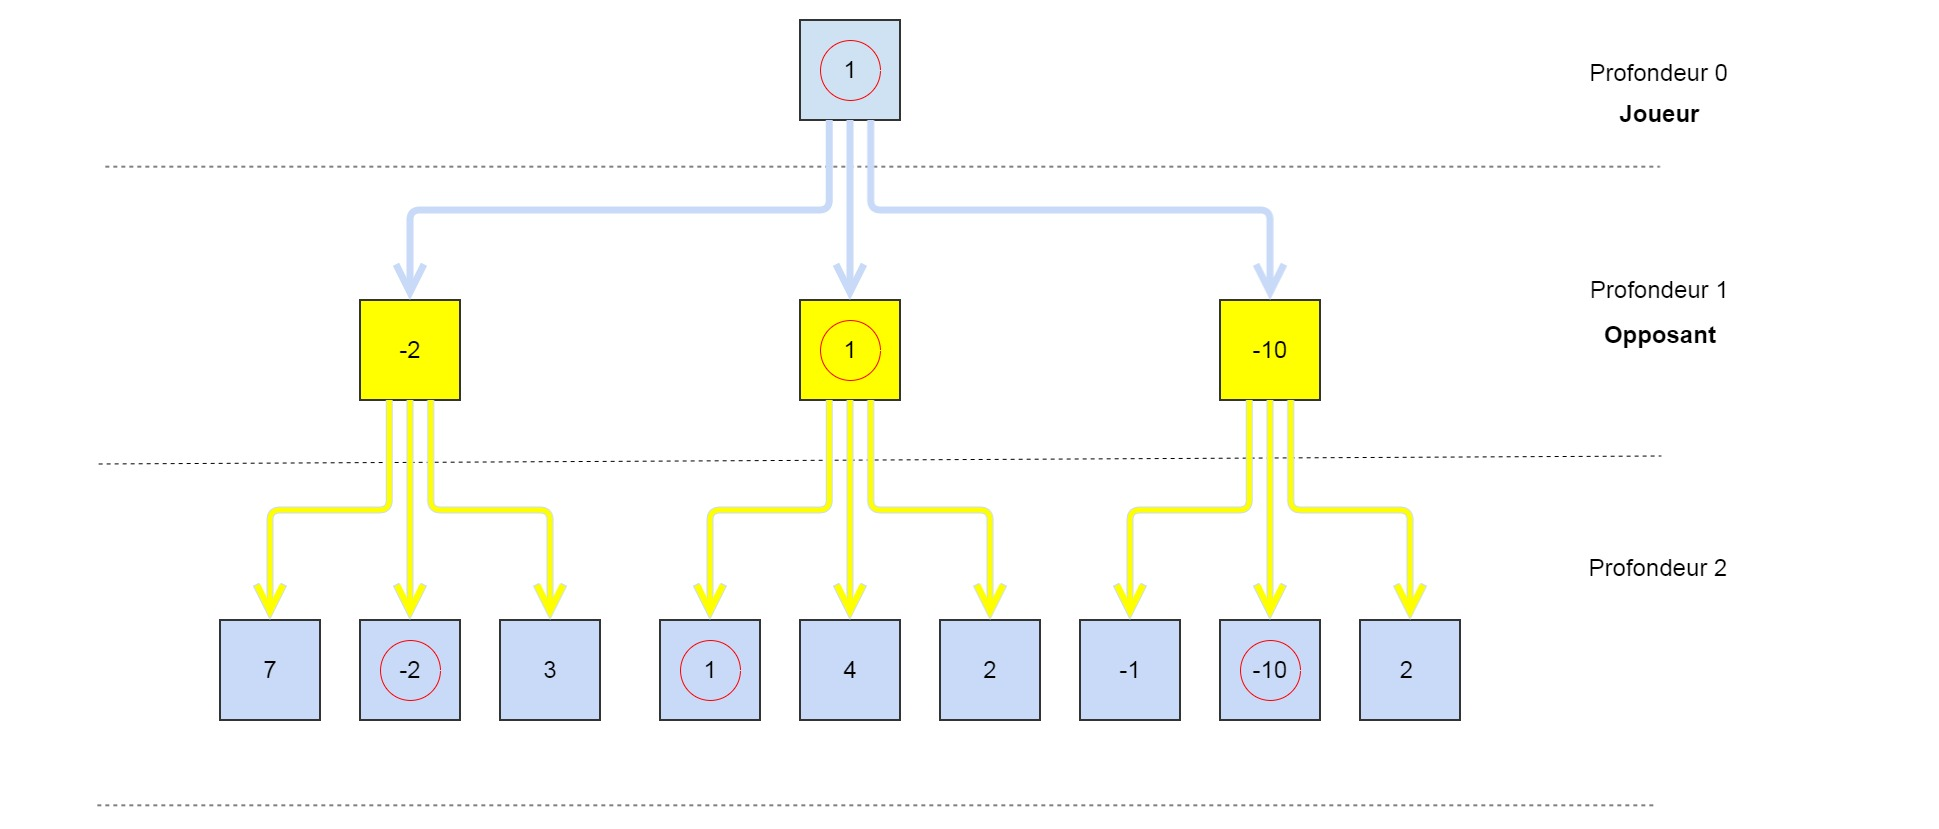
\includegraphics{images/minmax.jpg}
\caption{MiniMax}
\end{figure}

Sur le schéma suivant, les flèches bleues correspondent aux coups
possibles du joueur, les flèches jaunes à ceux de l'opposant.
L'algorithme est de profondeur 2 et on considère que trois coups sont
possibles pour chaque configuration de jeu.

L'algorithme va parcourir l'arbre et utiliser la procédure d'évaluation
pour associer à chaque feuille une valeur numérique. On se place ensuite
sur les noeuds de profondeur 1 qui prendra la valeur du plus petit de
ses fils : on minimise. On remonte ensuite d'un niveau et on prend ce
coup ci la valeur du plus grand des fils : on maximise.

On en déduit la série de coup la plus judicieuse à jouer : celle qui
mène à la feuille qui est remontée au niveau 0.

\begin{itemize}
\item
  p est le noeud d'un arbre, il possède n fils (f1, f2, \ldots{}, fn).
\item
  minimax(p) = eval(p) si p est une feuille
\item
  minimax(p) = max(minimax(f1), minimax(f2), \ldots{} minimax(fn)) si il
  s'agit d'un coup du joueur
\item
  minimax(p) = mim(minimax(f1), minimax(f2), \ldots{} minimax(fn)) si il
  s'agit d'un coup de son opposant
\end{itemize}

\subsection{Le Minimax associé aux
échecs}\label{le-minimax-associuxe9-aux-uxe9checs}

Le nombre de coup possible aux échecs pour un tour est élevé. Pour une
ouverture par exemple, au moins 20 coups différents sont possibles alors
que plusieurs pièces n'ont pas la possibilité de bouger. Ainsi pour
simuler les differentes possibilités sur les deux premiers tours on doit
evaluer prés de 400 coups et pour une profondeur de 3 : 8000 coups.
L'efficacité d'une IA Minimax est basée sur la profondeur de l'arbre des
coups. Par conséquent, notre algorithme devra travailler sur un arbre
relativement important et sera donc probablement coûteux en ressources.
Il nous faut donc optimiser l'implementation de notre algorithme Minimax
c'est pour cela que nous utiliserons l'elagage alpha-beta et une table
de transposition.

\subsection{L'evaluation d'un plateau de
jeu}\label{levaluation-dun-plateau-de-jeu}

la principale difficulté de l'algorithme minimax ainsi que son
efficacité repose sur la fonction d'evaluation, qui pour le jeux
d'echecs vas à partir de la configuration d'un échequier produire une
valeur numerique representant la pertinence de cette configuration. par
exemple lorsque le joueur adversaire est en echec l'evaluation de cette
configuration vas produire un trés grand nombre pour signaler que cette
position est favorable au joueur.

Nous allons donc basé l'evaluation d'un échequier sur differentes
données :

\begin{itemize}
\item
  Le nombre et le type de piéce present sur l'echequier :

  \begin{itemize}
  \itemsep1pt\parskip0pt\parsep0pt
  \item
    Il faudrait donc attribuer a chaque piéce une valeur en fonction du
    type de piéce et si lorsque la piéce est retirer du jeux, enlever
    cette valeur au score du plateau si la piéce appartient au joueur ou
    sinon l'ajouter si la piéce appartenait au joueur adverse.
  \end{itemize}
\item
  Comparer la configuration actuelle a des ouvertures connues :

  \begin{itemize}
  \itemsep1pt\parskip0pt\parsep0pt
  \item
    Nous disposons d'une base de données d'ouverture ou chaque
    connfiguration est représenté par un hash contenant la position et
    le type de toutes les piéces presente sur l'echequier, l'ensemble de
    ces hash serait donc placé dans une table de hashage et la fonction
    d'evaluation pourait donc ce reféré a cette base de donnnées en
    comparant le hash du jeu actuel avec celui de cette base de données
    d'ouverture.
  \end{itemize}
\item
  Prendre en compte les situations d'echecs et de pat

  \begin{itemize}
  \itemsep1pt\parskip0pt\parsep0pt
  \item
    L'evaluation doit absolument prendre en comptes les situations
    d'echecs, pat et mat notamement car l'echecs va bloquer la plupart
    des possibilité de jeu de l'adversaire car il est obligé de se
    sortir de cette situation mais plus encore c'est une conndition
    neccesaire à l'echecs et mat qui constitue le seul moyen de
    remporter la partie.
  \end{itemize}
\end{itemize}

\subsection{Optimisation du Min-Max}\label{optimisation-du-min-max}

\subsubsection{Le NégaMax}\label{le-nuxe9gamax}

Le principe du Negamax est relativement simple. Lorsque dans
l'algorithme min-max nous testons si nous sommes sur un noeud à niveau
pair ou impair, dans le but de maximiser ou de minimiser une évaluation,
le Négamax va toujours chercher à maximiser l'évaluation. Il suffit
d'inverser le signe des évaluations à chaque niveau, de ce fait, notre
algorithme va toujours chercher à maximiser une évaluation.

Ce principe est assez intérresant, car il nous permet d'alléger
l'algorithme min-max, en évitant certaines comparaisons.

\subsubsection{L'élagage Alpha-Beta}\label{luxe9lagage-alpha-beta}

L'algorithme Alpha-Beta est une amélioration de l'algorithme min-max. Le
but de cet algorithme est d'éviter le parcours de branches inutiles dans
l'arbre des coups possibles. Comme son noms l'indique, l'algorithme
alpha-beta utilise deux paramètres qui sont :

\begin{itemize}
\itemsep1pt\parskip0pt\parsep0pt
\item
  alpha;
\item
  beta.
\end{itemize}

La coupure alpha se fait sur les niveaux Min. Le principe de cette
coupure va être qui si la valeur d'un niveau Min est plus petite que la
valeur d'un niveau Max supérieur, nous considérons que la valeur du
noeud Max supérieur ne changera pas, de ce fait, il est inutile d'aller
explorer les branches suivantes du niveau Min.

D'un autre côté, nous avons la coupure béta, cependant, cette coupure
s'effectue sur les niveaux Max. Le principe de la coupure béta est le
même que pour la coupure alpha, mais pour les niveaux Max.

Nous avons donc deux coupures qui nous permettent d'éviter des parcours
inutiles dans l'arbre des coups possibles, ce qui est un gain de temps.

\subsubsection{Comment utiliser les variables alpha et béta
?}\label{comment-utiliser-les-variables-alpha-et-buxe9ta}

Tout d'abord, nous devons savoir qu'il y a deux règles :

\begin{itemize}
\itemsep1pt\parskip0pt\parsep0pt
\item
  sur un niveau max, si la valeur du noeud \textgreater{}= béta, nous
  effectuons une coupure béta (1);
\item
  sur un niveau min, si la valeur du noeud \textless{}= alpha, nous
  effectuons une coupure alpha (2).
\end{itemize}

C'est grâce à ces comparaisons quer nous pouvons effectuer un élagage,
alpha ou béta.

Les variables alpha et béta sont mis à jours lorsque un noeud retourne
une évaluation. Sur un niveau Min, la valeur béta va être mis à jour,
puis sur un noeud max, la valeur alpha va être mis à jour.

Toutes les valeurs alpha et béta vont remonter aux niveaux supérieurs,
et c'est à ce moment là que nous pourrons effectuer des tests avec les
règles (1) et (2), et donc procéder à des coupures si besoin. Il faut
savoir que les valeurs alpha et béta hérite des niveaux supérieurs.

\section{Ouverture}\label{ouverture}

Les ouvertures sont des stratétegies de jeux utilisées en debut de
parties, elle permettent notamment de bien positioner ses pièces et de
placer les rois en securités. Il existe une multitude d'ouvertures et
pour chacune d'entre-elles plusieurs variantes, elle sont souvent nommé
en fonction de leur inventeur.

On utilise la notation algebrique pour définir les ouvertures. Les
deplacements dans la colonne de gauche correspondent aux mouvements des
piéces blanches et ceux de la colonne de droite aux piéces de couleurs
noires.

\subsection{Implementation}\label{implementation}

Pour implémenter les bases de données d'ouverture nous avons choisis
d'utiliser une table de hachage. Un etat de l'échiquier sera donc
réprésenté par un hash et l'IA cherchera la correspondance entre l'etat
actuel de l'échiquier et une ouverture dans la base de données.

Format d'un hash :

(Initiale de la piéce - position sous la forme algebrique) : (suivant)
..

Example :

RA1:DA3:F2:C4

Correspond à :

\begin{itemize}
\itemsep1pt\parskip0pt\parsep0pt
\item
  Roi en position A1;
\item
  Dame en position A3;
\item
  Fou en position B2;
\item
  Cavalier en position C4.
\end{itemize}

Il faut respecter l'ordre dans lequelle sont placés les piéces dans le
hash afin que deux états identique aient toujours le même hash. On
définira donc l'ordre suivant :

Roi - Dame - Fou - Tour - Cavalier - Pion

Il faut aussi définir un ordre pour les piéces de même types. On peut
par exemple définir un ordre pour les cases :

Suggestions : - On compare les lettres A \textless{} B \textless{} C
\ldots{}; - Puis le nombre 1 \textless{} 2; - -\textgreater{} A8
\textless{} B2 \textless{} C3 \textless{} C6.

On aura donc bessoin :

\begin{itemize}
\itemsep1pt\parskip0pt\parsep0pt
\item
  D'une fonction comparant deux cases;
\item
  D'une fonction prenant une liste de piéce et renvoyant un hash.
\end{itemize}

\subsection{Defense Indienne}\label{defense-indienne}

Cette strategie permet de sécuriser la position de la reine pour le
joueur ayant les piéces noires.

\begin{enumerate}
\def\labelenumi{\arabic{enumi}.}
\itemsep1pt\parskip0pt\parsep0pt
\item
  : d4 Cf6
\item
  : c4 e6
\item
  : Cf3 b6
\end{enumerate}

\subsection{Defense Benoni}\label{defense-benoni}

\begin{enumerate}
\def\labelenumi{\arabic{enumi}.}
\itemsep1pt\parskip0pt\parsep0pt
\item
  : d4 Cf6
\item
  : c4 c5
\end{enumerate}

\subsection{Le mat du berger}\label{le-mat-du-berger}

Cette ouverture permet d'effectuer un echec et mat en seulement 4 tours.

\begin{enumerate}
\def\labelenumi{\arabic{enumi}.}
\itemsep1pt\parskip0pt\parsep0pt
\item
  : e4 e5
\item
  : Dh5 Cc6
\item
  : Fc4 Cf6
\item
  : Df7 -\textgreater{} Mat
\end{enumerate}

\subsection{La croisade du cavalier}\label{la-croisade-du-cavalier}

\begin{enumerate}
\def\labelenumi{\arabic{enumi}.}
\itemsep1pt\parskip0pt\parsep0pt
\item
  : d4 Cf6
\item
  : Cd2 e5
\item
  : de5 Cg4
\item
  : h3 Ce3 
\end{enumerate}

Pour réaliser ce projet, nous devons penser aux différentes structures,
types de données que nous allons utilisés dans notre projet.

\subsection{Structures de données}\label{structures-de-donnuxe9es}

\subsubsection{Représentation de
l'échiquier}\label{repruxe9sentation-de-luxe9chiquier}

Pour pouvoir réprésenter l'échiquier, nous allons implémenter une
structure représentant les cases de l'échiquier.

La structure ``Case'' sera donc la suivante :

\begin{lstlisting}
struct Case {
     int colonne;
     int ligne;
     Piece *piece;
}
\end{lstlisting}

\begin{itemize}
\itemsep1pt\parskip0pt\parsep0pt
\item
  L'entier colonne représente une colone de l'échiquier;
\item
  L'entier ligne représente une ligne de l'échiquier;
\item
  La structure Piece représente la pièce présente sur la case à la
  position colonne et ligne.
\end{itemize}

La structure ``Piece'' sera donc la suivante :

\begin{lstlisting}
struct Piece {
    char type;
    Case *case;
    Joueur *joueur;
}
\end{lstlisting}

\begin{itemize}
\itemsep1pt\parskip0pt\parsep0pt
\item
  Le char type représente le type de la pièce (pion, roi, dame, fou,
  tour);
\item
  La *case représente la case sur laquelle se trouve la pièce.
\item
  La *joueur permet d'avoir les différentes informations du joueur à qui
  appartient la pièce.
\end{itemize}

De ce fait, grâce à ces deux structures, nous pouvons représenter la
grille de notre échiquier.

La grille est donc : \lstinline!typedef Grille Case[8][8];!

Grâce à cette représentation, nous avons facilement accès aux pièces
présentent sur une case, ou à l'inverse, à la position d'une pièce dans
la grille.

\subsubsection{Représentation du
joueur}\label{repruxe9sentation-du-joueur}

De plus nous utiliserons une liste de Pièce qui va donc contenir les
différentes pièces encore présentent sur la grille, ce qui va nous être
utile pour effectuer des opérations sur l'ensemble des pièces, sans
faire de parcours inutile à partir de la grille. Par exemple, le calcul
de l'echec, ou du pat. Cette liste va être rattaché au joueur, pour
indiquer les pièces du joueur présente sur l'échiquier.

La structure ``Joueur'' sera donc la suivante :

\begin{lstlisting}

struct Joueur {
    int id;
    GList *listePieces;
    Piece *roi;
    Joueur* adverse;
    bool PrisePassant;
    Case *positionPrisePassant;
}
\end{lstlisting}

\begin{itemize}
\itemsep1pt\parskip0pt\parsep0pt
\item
  L'entier id représente le joueur 1 ou le joueur 2;
\item
  La Glist* listePieces représente la liste des pièces sur l'échiquier
  de joueur;
\item
  La Piece* roi permet de garder la position du roi en mémoire, pour
  calculer l'échec, et le pat plus rapidement;
\item
  Le Joueur* adverse permet d'avoir accès aux données du joueur adverse
  durant la partie;
\item
  Le booleen PrisePassant indique s'il est possible pour le joueur
  adverse d'effectuer une prise en passant pour le tour actuel.
\item
  La Case* positionPrisePassant permet de retenir l'endroit où il est
  possible d'effectuer une prise en passant.
\end{itemize}

\subsubsection{Représentation du jeu}\label{repruxe9sentation-du-jeu}

Pour représenter les différentes variables du jeu, nous allons les
regroupés dans une structure Jeu, qui va donc être :

\begin{lstlisting}
struct Jeu {
    Joueur* blanc;
    Joueur* noir;
    int tour;
    Grille* grille;
}
\end{lstlisting}

\begin{itemize}
\itemsep1pt\parskip0pt\parsep0pt
\item
  Le Joueur* blanc représente les pièces blanche;
\item
  Le Joueur* noir représente les pièces noires;
\item
  L'entier indique quel joueur doit jouer;
\item
  La Grille* grille représente la grille de l'échiquier.
\end{itemize}

\section{Implémentation du
déplacement}\label{impluxe9mentation-du-duxe9placement}

\subsection{Prototypes}\label{prototypes}

\begin{lstlisting}
/**
 * Permet d'effectuer le déplacement d'une pièce
 * 
 * g : Représente la grille du jeu, l'échiquier
 * depart :  Représente la case de départ de la pièce à déplacer
 * arrive :  Représente la case d'arrivée de la pièce déplacée
 * j : Représente le joueur
 *
 * retourne 0 si tout va bien, sinon un code d'erreur
 */

int deplacer(Grille* g,Case depart, Case arrive, Joueur* j);
\end{lstlisting}

\begin{lstlisting}
/**
 * Génère la liste des positions possibles pour une pièce
 * 
 * depart : Représente la case de la pièce a déplacer
 * retourne une Liste de doublé des positions possibles pour une pièce
 */     

GList* genererPosition(Case depart);
\end{lstlisting}

\begin{lstlisting}
/**
 * Vérifie les positions valide dans la GList* listePosition
 * 
 * listePosition : liste de doublé contenant toutes les positions possibles pour une pièce
 *  g : Représente la grille du jeu
 *  j : Représente un joueur 
 *  retourne la liste des déplacements valide (enlève les déplacements hors de la grille et sur les pions alliés)
 */

GList* check(GList* listePosition, Grille* g, Joueur* j);
\end{lstlisting}

\begin{lstlisting}

/**
 * Permet de mettre à jour les pièces déplacés et/ou mangés
 * 
 *  g : Représente la grille du jeu 
 *  listePosition :  liste de doublé contenant toutes les positions possibles pour une pièce
 *  depart : Représente la case de départ de la pièce 
 *  arrive : Représente la case d'arrivée de la pièce 
 *  j : Représente le joueur qui déplace sa pièce
 *
 */

void effectuerDeplacement(Grille* g, Glist* listePosition, Case depart, Case arrive, Joueur* j);
\end{lstlisting}

\begin{lstlisting}
/**
 * Permet d'annuler un déplacement d'une pièce
 * 
 * pieceDeplace : Représente la pièce qui a été déplacé
 * caseCible : Représente la case sur laquelle la pièce déplacé se trouvait
 * g : Représente la grille du jeu 
 * depart : Représente la case d'origine de la pièce déplacé
 */

void annulerDeplacement(Piece* pieceDeplace, Case* caseCible, Grille* g, Case* depart);
\end{lstlisting}

\begin{lstlisting}

/**
 * Permet d'annuler la prise de la pièce
 * 
 * piecePrise : Représente la pièce qui a été prisee
 * arrive : Représente la case sur laquelle était placé piecePrise
 * j : Représente le joueur
 */

void annulerPrise(Piece* piecePrise, Case* arrive, Joueur* j);
\end{lstlisting}

\begin{lstlisting}
/**
 * Permet de vérifier si le joueur j est en echec
 * On génère toutes les positions possibles des pièces, et on compare avec la liste de pièces du joueur

 * j : Représente le Joueur avec sa liste de pièce 
 * retourne vrai si le joueur est en echec, sinon retourne non
 */

bool isEchec(Joueur* j);
\end{lstlisting}

\subsection{Pseudo-code}\label{pseudo-code}

\begin{lstlisting}

int deplacer(Grille* g,Case *depart, Case *arrive, Joueur* j) {
    GList *p;
    p <- genererPosition(depart);
    p <- check(p,g,j);

    if (arrive in p) {
        Piece *pieceDeplacer;
        Piece *piecePrise = NULL;

        effectuerDeplacement(g,p,depart,arrive,j);

        if (isEchec(j)) {
            annulerDeplacement(pieceDeplace, arrive, g, depart);

            if (piecePrise) {
                annulerPrise(piecePrise, arrive, j);
            }

            return 1;
        }

    }
    return 0;
}


\end{lstlisting}

\section{Sauvegarde}\label{sauvegarde}

Le programme doit pouvoir sauvegarder l'etat d'une partie dans un
fichier de façon a pouvoir reprendre la partie entre chaque execution du
programme.

\subsection{Structure du fichier}\label{structure-du-fichier}

Nous devons stocker les données suivantes :

\begin{itemize}
\itemsep1pt\parskip0pt\parsep0pt
\item
  Les piéces :

  \begin{itemize}
  \itemsep1pt\parskip0pt\parsep0pt
  \item
    positions
  \item
    type
  \item
    appartenance joueurs
  \end{itemize}
\item
  l'avancement

  \begin{itemize}
  \itemsep1pt\parskip0pt\parsep0pt
  \item
    tours
  \end{itemize}
\item
  les joueurs :

  \begin{itemize}
  \itemsep1pt\parskip0pt\parsep0pt
  \item
    prisePassant
  \end{itemize}
\end{itemize}

Nous avons donc choisie de le modéliser de la facon suivante :

\begin{lstlisting}
{
    'Partie': {
        'Nombre de tours' : n,
        'PrisePassant': true/false,
        'PositionPrisePassant': 'A1 '
    },
    'Joueurs1': {
        'Hash': 'RA1:DB2...'
    },
    'Joueurs2': {
        'Hash': 'CA3:....'
    }
}
\end{lstlisting}

\section{Implementation}\label{implementation-1}

Deux choix on été retenue pour implémenter cette sauvegarde :

\begin{itemize}
\itemsep1pt\parskip0pt\parsep0pt
\item
  Fichier Binaire

  \begin{itemize}
  \itemsep1pt\parskip0pt\parsep0pt
  \item
    Avantage :

    \begin{itemize}
    \itemsep1pt\parskip0pt\parsep0pt
    \item
      Rapide à parcourir
    \item
      Petite taille du fichier
    \end{itemize}
  \item
    Incovenient

    \begin{itemize}
    \itemsep1pt\parskip0pt\parsep0pt
    \item
      Implementation
    \end{itemize}
  \end{itemize}
\item
  Fichier JSON

  \begin{itemize}
  \itemsep1pt\parskip0pt\parsep0pt
  \item
    Avantage

    \begin{itemize}
    \itemsep1pt\parskip0pt\parsep0pt
    \item
      Lecture facile
    \item
      Facilement utilisable par d'autres programmes
    \item
      Implementer par jsonGlib
    \end{itemize}
  \item
    Incovenient

    \begin{itemize}
    \itemsep1pt\parskip0pt\parsep0pt
    \item
      Taille importante des fichiers
    \end{itemize}
  \end{itemize}
\end{itemize}

\subsection{Prototype}\label{prototype}

\begin{lstlisting}
/**
 * Permet de sauvegarder dans un fichier l'état du jeu
 * 
 * fichier : Nom du fichier qui va être enregistré
 * jeu : Structure regroupant les joueurs, le tour, et la grille de l'échiquier
 * 
 * retourne 0 si tout va bien, sinon un code d'erreur si le fichier ne s'est pas enregistré
 */

int sauvegarder(char* fichier,Jeu* jeu);
\end{lstlisting}

\begin{lstlisting}
/**
 * Permet d'ouvrir un fichier et d'initialiser les variables associées
 * 
 * fichier : Nom du fichier qui va être chargé
 * jeu : Structure regroupant les joueurs, le tour, et la grille de l'échiquier
 * 
 * retourne 0 si tout va bien, sinon retourne un code d'erreur s'il y a une erreur lors du chargement du fichier
 */

int ouvrir(char* fichier, Jeu* jeu);
\end{lstlisting}

\end{document}
